\documentclass[17pt,xcolor=x11names]{beamer}
\usepackage[utf8]{inputenc}
\usepackage{tikz}
\usepackage{tkz-graph}
\usetikzlibrary{arrows,calc,automata,chains,matrix,positioning,scopes,decorations.pathmorphing}

\usecolortheme{seagull}
\useoutertheme{infolines}
\usefonttheme[onlymath]{serif}

\setbeamertemplate{headline}[default]
\setbeamertemplate{navigation symbols}{}
\mode<beamer>{\setbeamertemplate{blocks}[rounded][shadow=true]}
\setbeamercovered{transparent}
\setbeamercolor{block body example}{fg=blue, bg=black!20}

\newcommand\undermat[2]{%
  \makebox[0pt][l]{$\smash{\underbrace{\phantom{%
    \begin{matrix}#2\end{matrix}}}_{\text{$#1$}}}$}#2}

\title[Kép- és videofeldolgozás]{Kép- és videofeldolgozás}
\subtitle{}
\author[Kriván Bálint]{\textbf{Kriván Bálint} (\texttt{CBVOEN})\\[10pt]
\footnotesize Kovács Gábor (\texttt{kovacsg@tmit.bme.hu})}
\institute[BME]{}
\date{2013. dec. 12.}

\begin{document}

\begin{frame}\maketitle\end{frame}

\begin{frame}{Feladat}
\begin{itemize}
\item \textbf{Képrekonstrukció adott pontból}
\item OpenCV alapok
\item Kamera-kalibráció
\item Kamerák szinkronizációja
\end{itemize}
\end{frame}

\begin{frame}{OpenCV}
\begin{itemize}
\item Legelterjedtebb és legkiforrottabb
\item C++-ban íródott
\item API különböző nyelvekhez
\item nagyon jó dokumentáció
\end{itemize}
\end{frame}

\begin{frame}{,,Lyukkamera'' modell}
\[\small s \left[\begin{array}{c}
u \\ 
v \\
1
\end{array}\right] = \underbrace{\left[\begin{array}{ccc}
f_x & 0 & c_x \\ 
0 & f_y & c_y \\
0 & 0 & 1
\end{array}\right]}_{\mathbf{A}} \left[\begin{array}{ccc|c}
r_{11} & r_{12} & r_{13} & t_1 \\ 
r_{21} & r_{22} & r_{23} & t_2 \\
\undermat{\mathbf{R}}{r_{31} & r_{32} & r_{33}} & t_3 \\
\end{array}\right] \left[\begin{array}{c}
X \\ 
Y \\
Z \\
1
\end{array}\right]\]
\begin{itemize}
\item + torzítási együtthatók
\end{itemize}
\end{frame}

\begin{frame}{Félévi munka ismertetés 1.}
\begin{itemize}
\item kamera kalibráció
\begin{itemize}
\item \texttt{findChessboardCorners}
\item \texttt{calibrateCamera}
\end{itemize}
\end{itemize}

\begin{center}

\includegraphics[scale=0.10]{figs/pattern.png}
\end{center}

\end{frame}

\begin{frame}{Félévi munka ismertetés 2.}
\begin{itemize}
\item távoli feladat
\begin{itemize}
\item $n$ kamera vesz egy adott térrészt
\item választott pontba egy képzeletbeli kamera
\item mit látunk?
\end{itemize}
\item kamerák szinkronizációja
\item $\rightarrow$ lézerpont detekció
\end{itemize}
\end{frame}

\begin{frame}{Félévi munka ismertetés 3.}
\begin{itemize}
\item referencia kép
\end{itemize}
\begin{center}
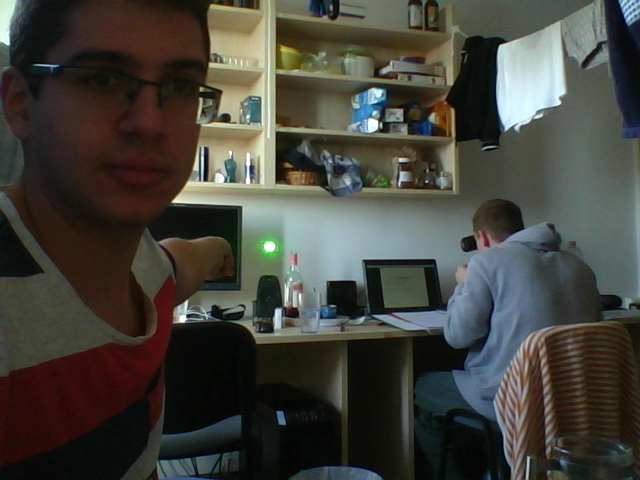
\includegraphics[scale=0.35]{figs/laser.png}
\end{center}
\end{frame}

\begin{frame}{Félévi munka ismertetés 4.}
\begin{itemize}
\item 1. algoritmus (átlós pixelek)
\end{itemize}
\begin{center}
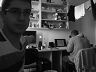
\includegraphics[scale=1.5]{figs/laser1-a.png}
\hspace{20pt}

\includegraphics[scale=1.5]{figs/laser1-b.png}
\end{center}
\end{frame}

\begin{frame}{Félévi munka ismertetés 5.}
\begin{itemize}
\item 2. algoritmus (négyzet)
\end{itemize}
\begin{center}
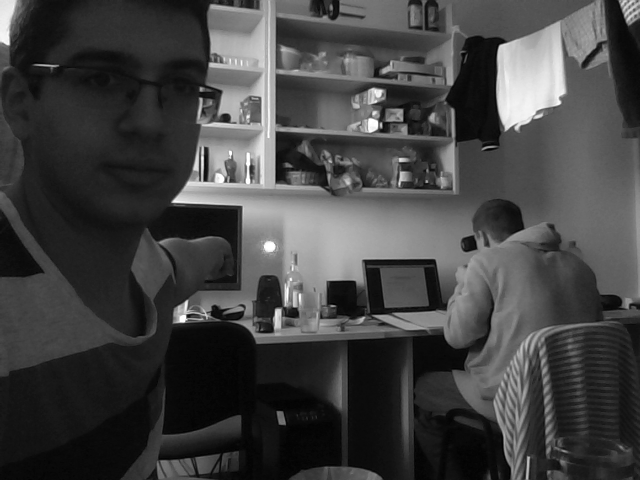
\includegraphics[scale=0.225]{figs/laser2-a.png}
\hspace{20pt}
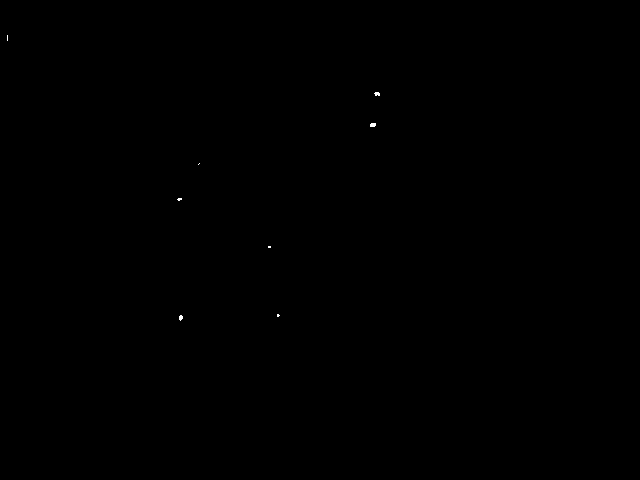
\includegraphics[scale=0.225]{figs/laser2-b.png}
\end{center}
\end{frame}

\begin{frame}{Félévi munka ismertetés 6.}
\begin{itemize}
\item 3. algoritmus (kör + aura)
\end{itemize}
\begin{center}
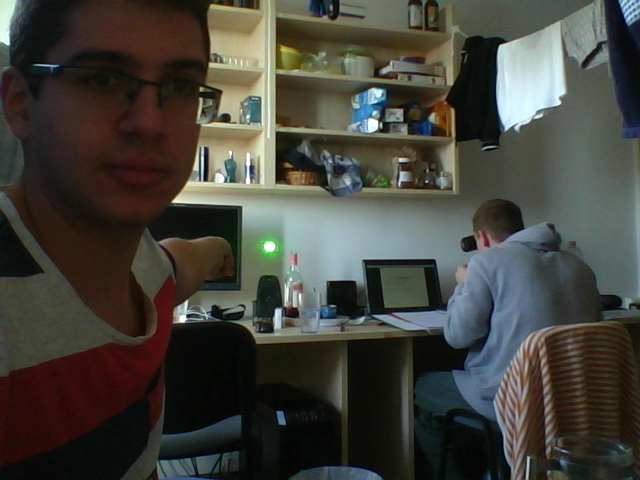
\includegraphics[scale=0.225]{figs/laser.png}
\hspace{20pt}
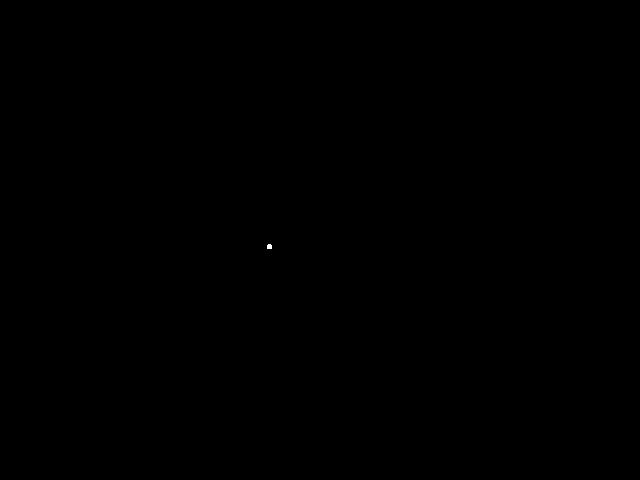
\includegraphics[scale=0.225]{figs/laser3-b.png}
\end{center}
\end{frame}

\begin{frame}{Félévi munka ismertetés 7.}
\begin{itemize}
\item 4. algoritmus (négyzet + aura)
\end{itemize}
\begin{center}
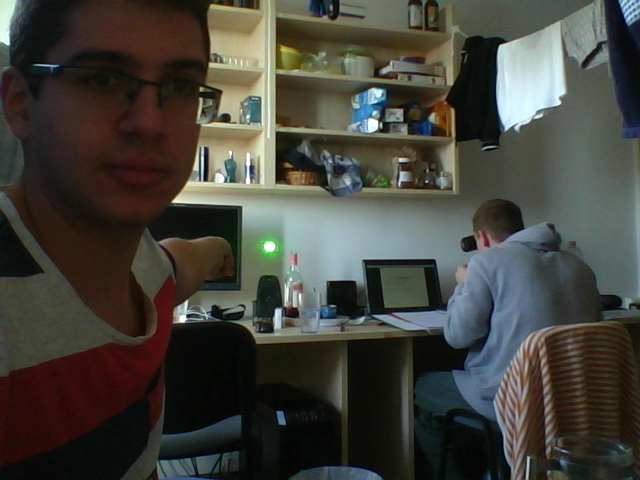
\includegraphics[scale=0.225]{figs/laser.png}
\hspace{20pt}
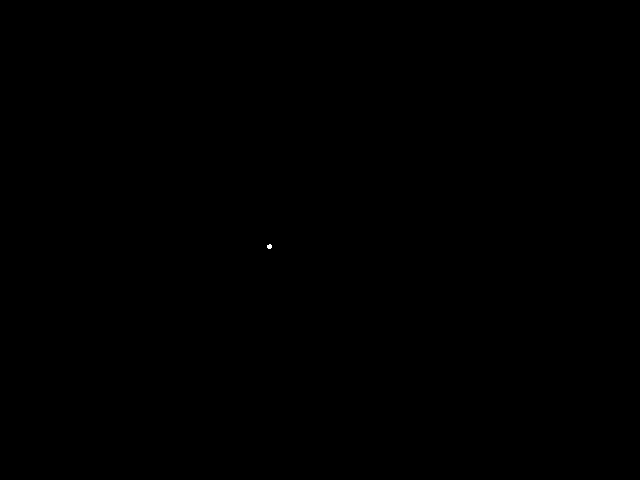
\includegraphics[scale=0.225]{figs/laser4-b.png}
\end{center}
\end{frame}

\begin{frame}{Összefoglalás és további tervek}
\begin{itemize}
\item OpenCV megismerése
\item kamera kalibrációja
\item lézerpont detekció\\\vspace{20pt}
\item lézerpont detekciója valós időben
\begin{itemize}
\item előre megadott helyen keressük a lézerpontot
\end{itemize}
\item képrekonstrukció egy választott pontból
\end{itemize}
\end{frame}

\end{document}